\chapter{Temperature sensor conditioning circuit}\label{sec:temp_sensor}

%**********************************************
\section{Intro} \label{sec:temp_intro_ch3}
%**********************************************
A temperature sensor needs a conditioning circuit that will allow the output of the sensor to be read by a micro-controller's ADC. This chapter will explain in detail how this circuit will be designed to meet the specific requirements of the Temperature sensor and the ADC. The design process is aided by the formulas found in \cite{Carter2002} and circuit descriptions in \cite{WebsiteOpAmp}.

%**********************************************
\section{Design}\label{sec:temp_design_ch3}
%**********************************************
The following parameters of the temperature sensor are specified as:\newline
\[V(\SI{0}{\celsius}) = \SI{620}{\milli\volt} ;\hspace{1em} \triangle V(+\SI{1}{\celsius}) = +\SI{20}{\milli\volt}\]
There are a couple of design requirements that must be adhered to. The circuit shall:
\begin{itemize}
\itemsep -1\parsep
    \item measure the output through the full range of \numrange{34}{42} \si{\celsius} which corresponds to a swing of greater than \SI{3.2}{\volt}
    \item suppress \SI{50}{\hertz} noise of \SI{10}{\milli\volt} amplitude to an accuracy of less than \SI{80}{\milli\volt}
    \item use less than \SI{25}{\milli\ampere}
    \item have a step response of less than \SI{100}{\milli\second} for a $\pm$\SI{1}{\celsius} change.
    \item simulate under 2 minutes in \texttt{LTSpice}.
\end{itemize}
From the parameters and the requirements, a linear equation can be formulated to used with \cite{Carter2002} to design the first steps of the differential amplifier circuit. Choosing $R_f$ as \SI{82}{\kilo\Omega}.
\[y = 20x+1.38\]
\[m= 1+\frac{R_f}{R_g} ; \hspace{1em} R_g = \frac{R_f}{m-1} = \frac{\SI{82}{\kilo\Omega}}{20-1}\approx\SI{4.3}{\kilo\Omega} \]
To determine the values of the voltage divider before the buffer, a divider circuit must be calculated from $R_g$ as if the buffer is not there. From these values, $R_1$ and $R_2$ can be calculated. $V_{ref}$ is equal to \SI{5}{\volt}
\[R_{g2} = \frac{R_g}{10} \approx \SI{430}{\kilo\Omega}; \hspace{1em} R_{g1} = R_g - R_{g2}\approx\SI{3.8}{\kilo\Omega}\]
\[V_{ref'} = \frac{|b|\times R_{g1}}{R_{g1}+R_f} = \SI{62}{\milli\volt}; \hspace{1em} R_1 = \frac{R_{g2}(V_{ref}-V_{ref'})}{V_{ref'}} \approx \SI{33}{\kilo\Omega}\]
\[R_2=\frac{V_{ref'}\times R_1}{V_{ref}-V_{ref'}}\approx\SI{430}{\Omega}\]

This concludes the basics of the differential amplifier. \par To use the whole swing of the amplifier, a virtual ground must be applied to the temperature signal. A simple voltage divider using 2 resistors of \SI{82}{\kilo\Omega} can be used to achieve this, along with a capacitor and tuning resistor that will allow us to center the virtual ground more effectively. The voltage divider network should give a \SI{2.5}{\volt} virtual ground. The capacitor also helps to slightly filter the input going into the differential amplifier, but is not necessary.\par
Lastly the output must be filtered to achieve the desired noise suppression, The amplified noise is now \SI{200}{\milli\volt}. The noise needs to be suppressed by at least \SI{-7.9}{\dB} in order to achieve the \SI{80}{\milli\volt} accuracy. Fortunately, a standard Low Pass Filter can be designed in \texttt{LTSpice} and adjusted to achieve the desired suppression. After the suppression is achieved, the filter will be tested to see if it still meets the step response requirement. For \SI{50}{\hertz} and $R_o = \SI{20}{\kilo\Omega}$ the capacitance is calculated as: 
\[C_o = \frac{1}{2\pi\times f_c \times R_o}=\frac{1}{2\pi \times 50 \times 20\si{\kilo}}\approx \SI{160}{\nano\farad}\]

\begin{figure}[H]
    \centering
    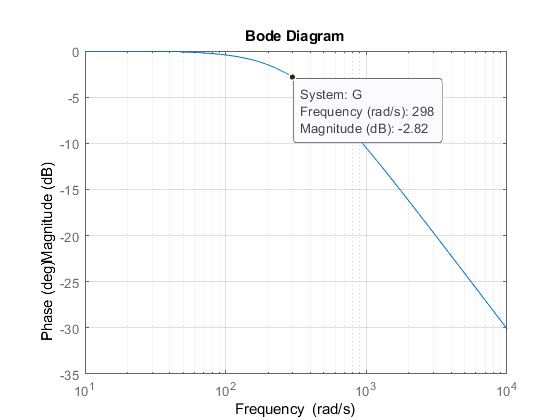
\includegraphics[width=0.7\linewidth]{./Figures/Pictures/LPFMatlab.png}
    \caption{LPF Bode Plot}
    \label{fig:lpf_bode}
\end{figure}
\newpage
%**********************************************
\section{Results} \label{sec:temp_results_ch3}
%**********************************************
The response of the system can be seen in Fig.\ref{fig:temp_circuit}. Once again, the current draw is measured using the\texttt{.meas} command in \texttt{LTSpice}.

\begin{figure}[H]
    \centering
    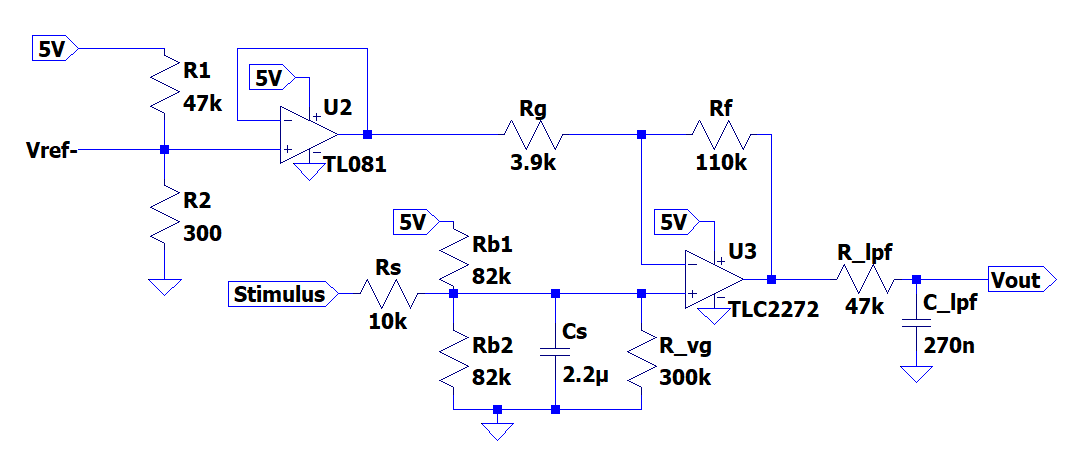
\includegraphics[width=\linewidth]{./Figures/Pictures/OPAMPFinal.png}
    \caption{Final Differential Op-amp circuit}
    \label{fig:opamp_final}
\end{figure}
\begin{figure}[H]
    \centering
    \begin{subfigure}[]{0.45\textwidth}
        \centering
  		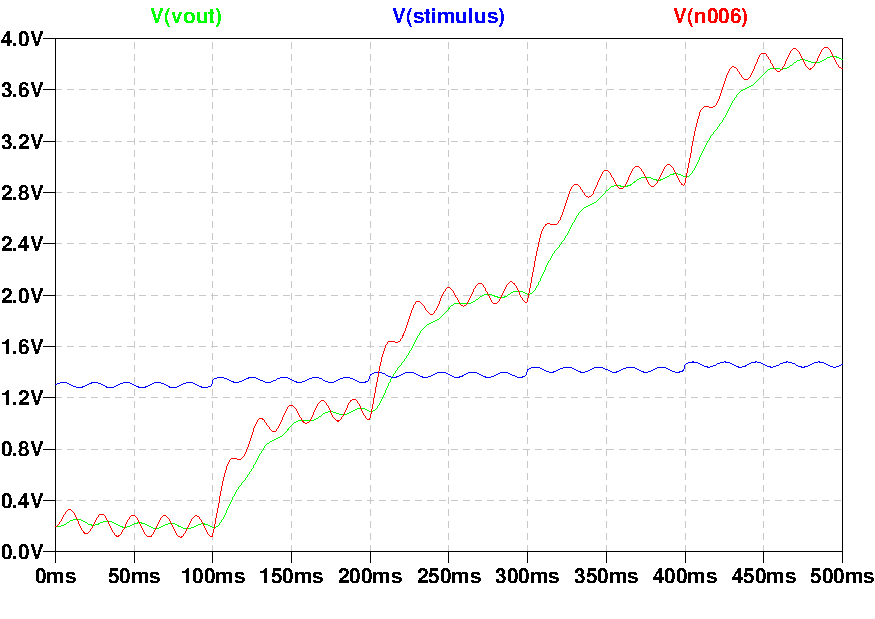
\includegraphics[width=1\linewidth]{./Figures/pdf/OpAmpStepResponse.pdf}
		\caption{} \label{subfig:opampresp}
    \end{subfigure}
    \begin{subfigure}[]{0.45\textwidth}
        \centering
  		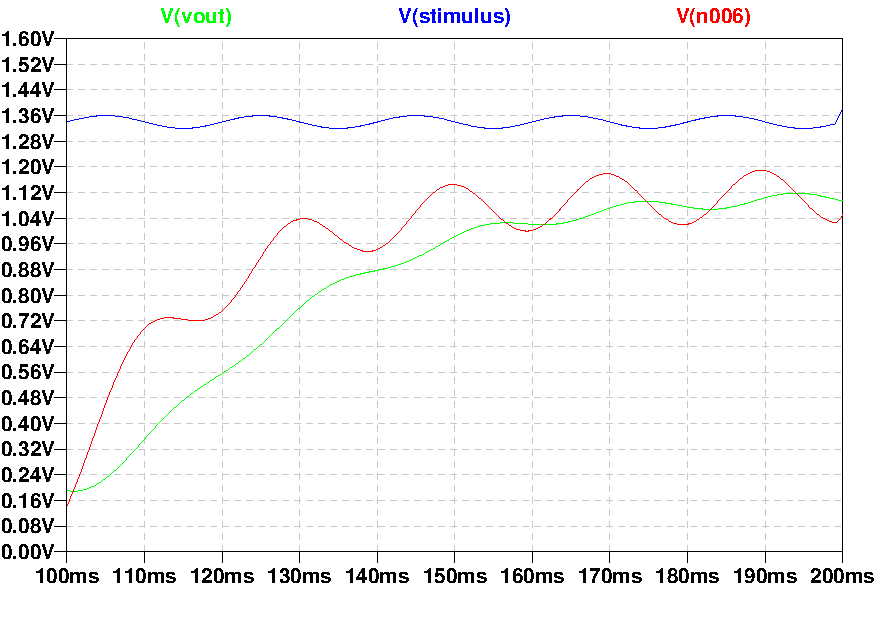
\includegraphics[width=1\linewidth]{./Figures/pdf/OpAmpStepResponse100ms.pdf}
		\caption{} \label{subfig:opamprespzoom}
    \end{subfigure}
    \begin{subfigure}[]{0.45\textwidth}
        \centering
  		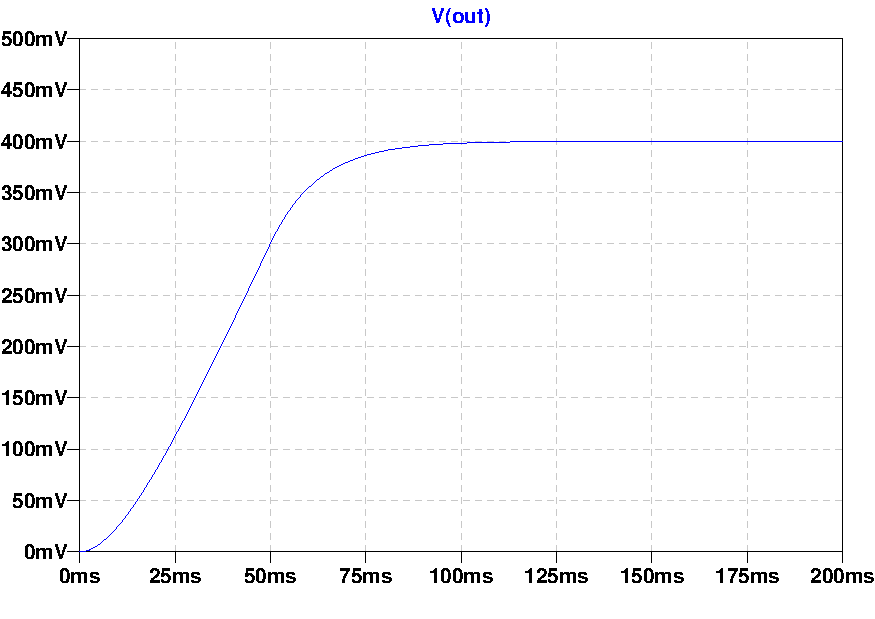
\includegraphics[width=1\linewidth]{./Figures/pdf/LPFResponse2.pdf}
		\caption{} \label{subfig:lpfresp}
    \end{subfigure}
    \begin{subfigure}[]{0.45\textwidth}
        \centering
  		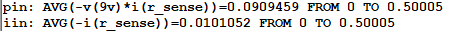
\includegraphics[width=1\linewidth]{./Figures/Pictures/OpAmpMeasResults.png}
		\caption{} \label{subfig:opampcurr}
    \end{subfigure}
    \caption{Temperature Condition Circuit outputs..(a) Output vs Input vs Unfiltered Output  (b) Zoomed 100ms partition of \ref{subfig:opampresp} (c) Simulated LPF response (c) Circuit total current draw \texttt{.meas} results}
    \label{fig:temp_circuit}
\end{figure}

\begin{table}[H]
    \centering
    \footnotesize
    \captionsetup{justification=centering}
    \caption{Table of time taken to finish simulation \\}
    \begin{tabular}{c@{\qquad}r}
    \toprule
         \multirow{3}{*}{Simulation Time-frame} & Total Simulation\\
         & Elapsed Time \\
    \midrule
         \SI{500}{\milli\second} & \SI{3.954}{\second}\\
    \bottomrule
    \end{tabular}
    \label{tab:sim_time}
\end{table}
\par
From the results it can be seen that the circuit meets the requirements. From Fig.\ref{subfig:opampresp} it can be seen that the circuit takes advantage of the full swing of the op-amp. allowing a response between roughly \numrange{3.8}{0.2} \si{\volt}. In Fig.\ref{subfig:opamprespzoom} it can be seen that the circuit achieves the 100ms rise time as set out bu the requirements. The LPF adheres to the step response as well in Fig.\ref{subfig:lpfresp}. The circuit draws less than \SI{15}{\milli\ampere} on average and simulates under 2 minutes on the machine used.
%**********************************************
\section{Summary}\label{sec:temp_summary_ch3}
%**********************************************
In summary, the circuit adheres to the requirements, while also improving on some. The output swing is greater than the designed \SI{3.2}{\volt} and only uses \SI{10.1}{\milli\ampere}. Although the rise time of the LPF could be designed to be more responsive, it meets the requirements without the need of a more complex LPF like a Butterworth-filter. This circuit meets the requirements all while only using 2 op-amps.


